% !TEX TS-program = xelatex
% !TEX encoding = UTF-8 Unicode

\documentclass[mathserif,11pt,aspectratio=169]{beamer}


\usetheme{Comet}


% Font setting 
\usepackage{fontspec}
\usepackage{xetexko}
\setmainhangulfont[BoldFont={Pretendard Bold}]{Pretendard Light}
\setsanshangulfont[BoldFont={Pretendard Bold}]{Pretendard Light}

\setbeamerfont{title}{family=\fontspec{Montserrat}}
\setbeamerfont{frametitle}{family=\fontspec{Montserrat},series=\bfseries, size=\LARGE}
\setbeamerfont{title page title}{family=\fontspec{Montserrat}, series=\bfseries, size=\huge} \setbeamerfont{title page author}{family=\sffamily, series=\bfseries, size=\Large}   
\setbeamerfont{title page logo}{family=\fontspec{Montserrat}, size=\footnotesize}   
\setbeamerfont{sectionsubtitle}{family=\sffamily, size=\large}   
\setbeamerfont{page number}{family=\fontspec{Montserrat}, series=\bfseries, size=\tiny}  


\title{KAIST ISE COMET Lab Presentation Slide Template}
\author{Changhyun Kwon\\권창현}




%%%%%%%%%%%%%%%%%%%%%%%%%%%%%%%%%%%%%%%%%%%%%%%%%%%%%%%%%%%%%%%%%%%%%
% Custom Packages and Macros
%%%%%%%%%%%%%%%%%%%%%%%%%%%%%%%%%%%%%%%%%%%%%%%%%%%%%%%%%%%%%%%%%%%%%

\usepackage{mwe}
\usepackage{amsmath}
\usepackage{amsfonts}
\usepackage{amssymb}
\usepackage{graphicx}
\usepackage{multicol}
\usepackage{multirow}
\usepackage{color}
\usepackage{natbib}
\usepackage{booktabs}
\usepackage{bbold}
\usepackage{tikz}
\usetikzlibrary{positioning,shapes,shadows,arrows}

\usepackage{etoolbox}
\makeatletter
\def\do#1{\@namedef{#1c}{\ensuremath{\mathcal{#1}}}}
\docsvlist{A,B,C,D,E,F,G,H,I,J,K,L,M,N,O,P,Q,R,S,T,U,V,W,X,Y,Z}
\makeatother

\makeatletter
\def\do#1{\@namedef{#1b}{\ensuremath{\mathbb{#1}}}}
\docsvlist{A,B,C,D,E,F,G,H,I,J,K,L,M,N,O,P,Q,R,S,T,U,V,W,X,Y,Z}
\makeatother

\newcommand{\red}[1]{{\color{red}#1}}
\newcommand{\blue}[1]{{\color{blue}#1}}
\newcommand{\green}[1]{{\color{green!60!white}#1}}

\newcommand{\email}[1]{{\href{mailto:#1}{\nolinkurl{#1}}}}

\usepackage{bm}
\renewcommand{\vec}[1]{\boldsymbol{\mathbf{#1}}}
\newcommand{\mat}[1]{\vec{#1}}
\newcommand{\set}[1]{\boldsymbol{\mathbf{#1}}}
\newcommand{\optset}[1]{\mathbb{#1}}

%\renewcommand{\bar}[1]{\mkern 1.5mu\overline{\mkern-1.5mu#1\mkern-1.5mu}\mkern 1.5mu}
%\renewcommand{\hat}{\widehat}
%\renewcommand{\tilde}{\widetilde}

\newcommand{\ds}{\mathop{}\!\mathrm{d}s}
\newcommand{\dx}{\mathop{}\!\mathrm{d}x}
\newcommand{\dy}{\mathop{}\!\mathrm{d}y}
\newcommand{\dz}{\mathop{}\!\mathrm{d}z}
\newcommand{\dt}{\mathop{}\!\mathrm{d}t}
\DeclareMathOperator{\ord}{ord}

\DeclareMathOperator*{\minimize}{minimize}
\DeclareMathOperator*{\maximize}{maximize}
\DeclareMathOperator*{\argmax}{\arg \max}
\DeclareMathOperator*{\argmin}{\arg \min}
\DeclareMathOperator*{\conv}{conv}

\newtheorem{proposition}{Proposition}

%%%%%%%%%%%%%%%%%%%%%%%%%%%%%%%%%%%%%%%%%%%%%%%%%%%%%%%%%%%%%%%%%%%%%


\everymath{\displaystyle}

\begin{document}




%!TEX root = comet_beamer_example.tex


% Title page
\frame[plain]{\titlepage}


\begin{frame}
    \frametitle{Title and Content (default)}
    \Large
    \begin{itemize}
    \item Sleeping in his car was never the plan but sometimes things don't work out as \textbf{planned}. 한글 한글 This had been his life for the last three months and he was just beginning to get used to it. He didn't actually enjoy it, but he had accepted it and come to terms with it. Or at least he thought he had. All that changed when he put the key into the ignition, turned it and the engine didn't make a \textbf{sound}.
    \item 한글은 이렇게 보입니다. English랑 섞어 쓰기. \textbf{두꺼운 글씨체.}
    \end{itemize}
\end{frame}


\begin{frame}
    \frametitle{\comet Title and Content (comet)}
    \Large
    \begin{itemize}
    \item Sleeping in his car was never the plan but sometimes things don't work out as \textbf{planned}. 한글 한글 This had been his life for the last three months and he was just beginning to get used to it. He didn't actually enjoy it, but he had accepted it and come to terms with it. Or at least he thought he had. All that changed when he put the key into the ignition, turned it and the engine didn't make a \textbf{sound}.
    \item 한글은 이렇게 보입니다. English랑 섞어 쓰기. \textbf{두꺼운 글씨체.}
    \end{itemize}
\end{frame}

\begin{frame}
    \frametitle{\nub Title and Content (nub)}
    \Large
    \begin{itemize}
    \item Sleeping in his car was never the plan but sometimes things don't work out as \textbf{planned}. 한글 한글 This had been his life for the last three months and he was just beginning to get used to it. He didn't actually enjoy it, but he had accepted it and come to terms with it. Or at least he thought he had. All that changed when he put the key into the ignition, turned it and the engine didn't make a \textbf{sound}.
    \item 한글은 이렇게 보입니다. English랑 섞어 쓰기. \textbf{두꺼운 글씨체.}
    \end{itemize}
\end{frame}

\begin{frame}
    \frametitle{\geese Title and Content (geese)}
    \Large
    \begin{itemize}
    \item Sleeping in his car was never the plan but sometimes things don't work out as \textbf{planned}. 한글 한글 This had been his life for the last three months and he was just beginning to get used to it. He didn't actually enjoy it, but he had accepted it and come to terms with it. Or at least he thought he had. All that changed when he put the key into the ignition, turned it and the engine didn't make a \textbf{sound}.
    \item 한글은 이렇게 보입니다. English랑 섞어 쓰기. \textbf{두꺼운 글씨체.}
    \end{itemize}
\end{frame}

\begin{frame}
    \frametitle{\cross Title and Content (cross)}
    \Large
    \begin{itemize}
    \item Sleeping in his car was never the plan but sometimes things don't work out as \textbf{planned}. 한글 한글 This had been his life for the last three months and he was just beginning to get used to it. He didn't actually enjoy it, but he had accepted it and come to terms with it. Or at least he thought he had. All that changed when he put the key into the ignition, turned it and the engine didn't make a \textbf{sound}.
    \item 한글은 이렇게 보입니다. English랑 섞어 쓰기. \textbf{두꺼운 글씨체.}
    \end{itemize}
\end{frame}

\begin{frame}
    \frametitle{\nubexp Title and Content (nubexp)}
    \Large
    \begin{itemize}
    \item Sleeping in his car was never the plan but sometimes things don't work out as \textbf{planned}. 한글 한글 This had been his life for the last three months and he was just beginning to get used to it. He didn't actually enjoy it, but he had accepted it and come to terms with it. Or at least he thought he had. All that changed when he put the key into the ignition, turned it and the engine didn't make a \textbf{sound}.
    \item 한글은 이렇게 보입니다. English랑 섞어 쓰기. \textbf{두꺼운 글씨체.}
    \end{itemize}
\end{frame}






\begin{frame}

   \begin{block}{This is a Block}
      This is important information
   \end{block}

\pause

   \begin{alertblock}{This is an Alert block}
   This is an important alert
   \end{alertblock}

\pause

   \begin{exampleblock}{This is an Example block}
   This is an example 
   \end{exampleblock}

\end{frame}

%%%%%%%%%%%%%%%%%%%%%%%%%%%%%%%%%%%

\begin{frame}
\frametitle{SLIDE TITLE... 한글 제목 Slide Title}

Hello $\int_0^x y \dy$ \alert<2>{ddd}
\begin{itemize}
\item Queen $x^2 + y^2 = z^2$
\item Hello World $\mat{A}^\top \vec{x} = \vec{0}$
\item Good Morning $a\in\Ac$, $n\in\Nc$, $\Bb$, $\Eb$
\item Good Night $\sum_{(i,j)\in\Ac} x_{ij} y_{ij} \leq 1$ 
\item 안녕하세요 \textbf{굵은 글씨} $\textstyle\sum_{i=1}^n x_i = 1$
\end{itemize}

\begin{itemize}
\item<1-> Hello \alert{World}
\item<2-> Good \alert{Morning}
\item<3-> Good \alert{Night}
\end{itemize}

\end{frame}


\begin{frame}
\frametitle{\comet Bin Packing Problem}
A binary integer program can be formulated as follows:
\begin{align}
Z^* = \min_{\vec{z}} \ & \sum_{k\in\Kc} z_k \\
\text{s.t.} \ 
& \color{red}\sum_{k\in\Kc} y_{ik} = 1 \quad \forall i\in\Ic && (\lambda_i) \label{pack_once} \\
& \color{blue}\sum_{i\in\Ic} D_i y_{ik} \leq V z_k \quad \forall k\in\Kc \\
& y_{ik} \in \{0, 1\} \quad \forall i\in\Ic, k\in\Kc\\
& z_k \in \{0, 1\} \quad \forall k\in\Kc
\end{align}
where $\vec{\lambda}$ is a vector of Lagrangian multipliers for constraints \eqref{pack_once}.
The binary variable $y_{ik}$ is one if item $i$ is packed in $k$ and zero otherwise, and $z_k$ is one if bin $k$ is used.

\end{frame}



\begin{sectionframe}{
        Section Frame Title is Here. You can use this as a paper title and a very long title.
    }{
        Sobhanan, A., Park, J., Park, J. and Kwon, C., 2024. Genetic algorithms with neural cost predictor for solving hierarchical vehicle routing problems. Transportation Science.
    }
    \vspace{1cm}
    \begin{flushright}
        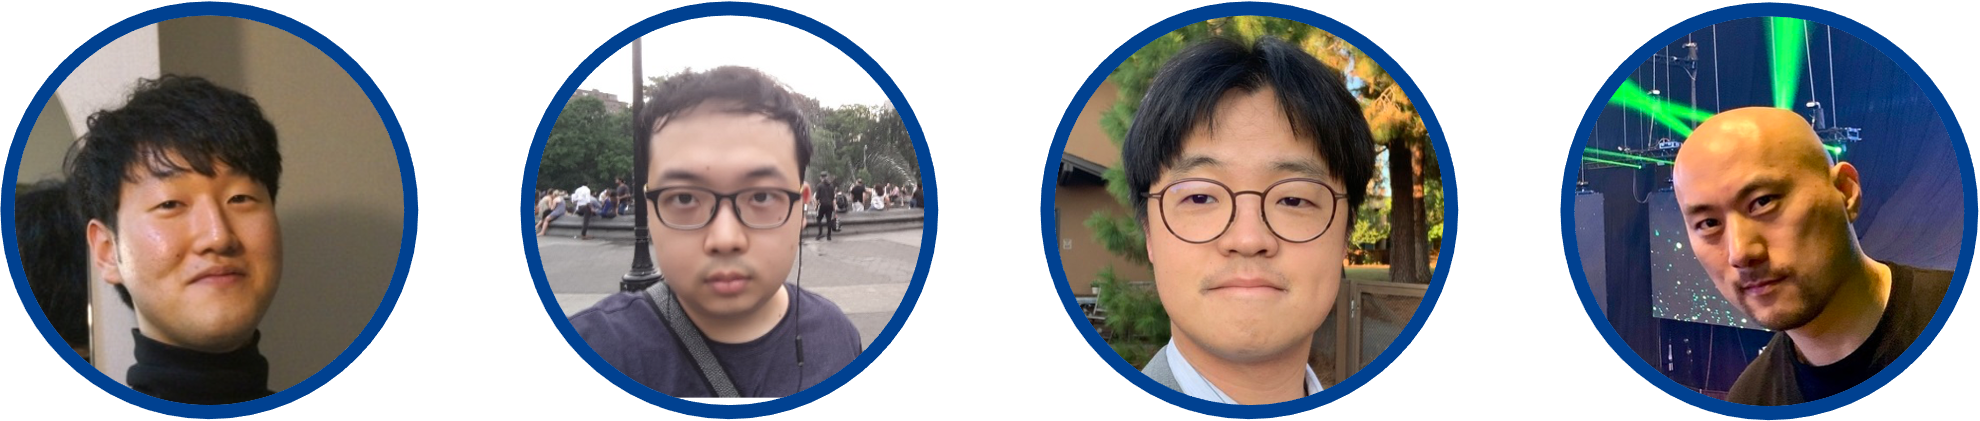
\includegraphics[width=7cm]{faces.png}
    \end{flushright}
\end{sectionframe}

\begin{sectionframe}{\nubexp Numerical Experiments}{}
\end{sectionframe}


\begin{frame}
\frametitle{LISTS...}
\texttt{itemize:}
\begin{itemize}
\item Hello \alert{World}
\item Good \alert{Morning}

  \begin{itemize}
  \item Hello \alert{World}
  \item Good \alert{Morning}
  
    \begin{itemize}
    \item Hello \alert{World}
    \item Good \alert{Morning}
    \end{itemize}
  
  \end{itemize}

\end{itemize}


\texttt{enumerate:}
\begin{enumerate}
\item Hello World
\item Good Morning
\end{enumerate}

\texttt{description:}
\begin{description}
\item [Hello] World
\item [Good] Morning
\end{description}

\end{frame}


\begin{frame}
\frametitle{\comet Research Areas}
\texttt{tikz} figure:

\definecolor{blue3}{HTML}{004191}
\definecolor{brown3}{HTML}{7a6847}
\definecolor{orange3}{HTML}{faa913}

\centering
\begin{tikzpicture}[scale=0.7, transform shape]

    \begin{scope}[blend group = screen]
      \fill[blue3!50!white] (90:1.8) circle (2.5);
      \fill[brown3!50!white] (210:1.8) circle (2.5);
      \fill[orange3!50!white] (330:1.8) circle (2.5);
    \end{scope}

	\draw[blue3] (90:1.8) circle (2.5);
	\draw[brown3] (210:1.8) circle (2.5);
	\draw[orange3] (330:1.8) circle (2.5);


    \node [font=\bf] at (90:2.5) {Transportation};
    \node [font=\bf] at (210:2.7) {Optimization};
    \node [font=\bf] at (330:2.7) {Computation};
%    \node [font=\Large] {Data Science};

	\begin{scope}[shift={(90:1.8 )}]
    	\node [font=\footnotesize, anchor=west] at ( 60:2.7 ) {Last-Mile Delivery};
    	\node [font=\footnotesize, anchor=west] at ( 38:2.7 ) {Urban Logistics};
    	\node [font=\footnotesize, anchor=west] at ( 20:2.7 ) {Risk Management};
    
    	\node [font=\footnotesize, anchor=east] at ( 120:2.7 ) {Market Design};
    	\node [font=\footnotesize, anchor=east] at ( 142:2.7 ) {Shared Mobility};
    	\node [font=\footnotesize, anchor=east] at ( 160:2.7 ) {EV Infrastructure};
	\end{scope}
	
	\begin{scope}[shift={(210:1.8 )}]
    	\node [font=\footnotesize, anchor=east] at ( 155:2.7 ) {Network Optimization};
    	\node [font=\footnotesize, anchor=east] at ( 175:2.7 ) {Bilevel Optimization};
    	\node [font=\footnotesize, anchor=east] at ( 195:2.7 ) {Robust Optimization};
    	\node [font=\footnotesize, anchor=east] at ( 215:2.7 ) {Equilibrium Models};	
    	\node [font=\footnotesize, anchor=east] at ( 235:2.7 ) {Game Theory};	
	\end{scope}

	\begin{scope}[shift={(330:1.8 )}]
    	\node [font=\footnotesize, anchor=south west, align=left] at ( 20:2.7 ) {Large-Scale Optimization\\Algorithms};
    	\node [font=\footnotesize, anchor=west, align=left] at ( 2:2.7 ) {Neural Combinatorial\\Optimization};
    	\node [font=\footnotesize, anchor=west] at ( -20:2.7 ) {Machine Learning};	
    	\node [font=\footnotesize, anchor=west] at ( -38:2.7 ) {Hybrid Algorithms};	
		\node [font=\footnotesize, anchor=west] at ( -60:2.7 ) {Open-Source Software};
	\end{scope}



\end{tikzpicture}
\end{frame}


\begin{frame}
\frametitle{\nub Theorems}

\begin{theorem}[Necesssary Condition]
Let $\vec{\lambda}^* = \argmax_{\vec{\lambda}} g(\vec{\lambda})$ and $\vec{x}^*$ is the corresponding knapsack solution.
We have
\begin{equation} \label{eq_partial_convexity}
	\sum_{i\in\Ic} \lambda^*_i x^*_i = 1.
\end{equation}
This also implies $\lambda^*_i \in [0, 1]$ for all $i\in\Ic$.
\end{theorem}

This theorem is... 

\pause 

\begin{lemma}
Hello theorem
\[
	1 + 2 = 3
\]
\end{lemma}

This lemma is ... 

\end{frame}



\begin{frame}
\frametitle{\cross Theorems}

\begin{theorem}
Hello theorem, you can put ``pause'' anywhere
\pause
\[
	\sum_{i=1}^n x_i = 1
\]
\end{theorem}
\end{frame}












\begin{frame}
\frametitle{Image Overlay}
\begin{center}
\includegraphics<1>[width=0.6\textwidth]{example-image-a}
\includegraphics<2>[width=0.6\textwidth]{example-image-b}
\includegraphics<3>[width=0.6\textwidth]{example-image-c}
\end{center}
\end{frame}


 

%%%%%%%%%%%%%%%%%%%%%%%%%%%%%%%%%%%
%%%%%%%%%%%%%%%%%%%%%%%%%%%%%%%%%%%

\begin{frame}
\frametitle{GOODBYE}

Goodbye world. \email{chkwon@kaist.ac.kr}

\begin{center}

\includegraphics[width=5cm]{logos/comet-logo-white-bg.pdf}
\quad 
\includegraphics[width=5cm]{logos/comet-logo.pdf}
\end{center}

\vspace*{\fill} 

\begin{center}
\scriptsize
\textbf{CREDIT:} KAIST Characters by 김태수, 석현정, KAIST Brand Shop. 
\raisebox{-0.2cm}{%

\includegraphics[height=0.7cm]{logos/nub.jpg}%

\includegraphics[height=0.7cm]{logos/geese.png}%
}
\end{center}
\end{frame}






\end{document}